\documentclass[a4paper, 12pt]{article}

\usepackage[english,russian]{babel}
\usepackage[T2A]{fontenc}
\usepackage[utf8]{inputenc}
\usepackage{geometry}
\usepackage{enumitem}
\usepackage{setspace}
\usepackage{amssymb}
\usepackage{graphicx}
\usepackage{wrapfig}
\usepackage{float}
\usepackage{amsmath}
\usepackage{textcomp}
\usepackage{dsfont}

\geometry{top=5mm, left=1cm}
%\setlength{\parindent}{0}
\renewcommand{\arraystretch}{1.2}
\linespread{1}

\begin{document}
    \begin{center}
        \textbf{Сферическая геометрия №1}\\
        Сечения сферы
    \end{center}

    \begin{center}
        \textbf{№1}
    \end{center}

    Что получиться в сечении сферы радиуса $R$ плоскостью, удаленной от центра сферы на $H$, если:\\
    \begin{minipage}[t]{0.5\textwidth}
        \begin{enumerate}
            \setcounter{enumi}{0}
            \item $R = 5$ см, $H = 6$ см.\\
            Ответ: не пересекаются

            \item $R = 2$ см, $H = 2$ см.\\
            Ответ: точка

            \item $R = 4$ см, $H = 1$ см.\\
            Ответ: окружность

            \item $R = 4$ см, $H = \sqrt {15}$ см.\\
            Оценка:
            \[ 4 \ ? \ \sqrt{14} \]
            \[ 16 \ ? \ 14  \]
            \[ 16 > 14 \rightarrow 4 > \sqrt{14}  \]
            Ответ: окружность

            \item $R = 5,65$ см,$H = \sqrt{32}$ см.\\
            Оценка:
            \[ 5,65 \ ? \ \sqrt{32}\]
            \[ 31,9225 \ ? \ 32 \]
            \[ 31,9225 < 32 \rightarrow 5,65 < \sqrt{32}\]
            Ответ: не пересекаются

            \item $R = 1$ см, $H = (\sqrt{2} + 5)^{\sqrt{4}\left(\frac{2}{\sqrt{2}} - \sqrt{2}\right)}$ см.\\
            Оценка:
            \[  (\sqrt{2} + 5)^{\sqrt{4}\left(\frac{2}{\sqrt{2}} - \sqrt{2}\right)} =
            (\sqrt{2} + 5)^{\sqrt{4}\left(\frac{2 - 2}{\sqrt{2}}\right) }  =\]
            \[(\sqrt{2} + 5) ^ 0 = 1 \rightarrow 1 = (\sqrt{2} + 5)^{\sqrt{4}\left(\frac{2}{\sqrt{2}} - \sqrt{2}\right)}\]
            Ответ: точка
        \end{enumerate}
    \end{minipage}
    \begin{minipage}[t]{0.5\textwidth}
        \begin{enumerate}
            \setcounter{enumi}{6}
            \item $R = 2 ^ {100}$ см, $H = 100 ^ 2$ см.\\
            Оценка:
            \[ 2 ^ {100} \ ? \ 100 ^ 2  \]
            \[ 2 ^ {50} \ ? \ 100 \]
            \[2 ^ {25} \ ? \ 10\]
            \[1024 * 2 ^ {15} \ ? \ 10 \]
            \[1024 * 2 ^ {15} > 10 \rightarrow 2 ^ {100} > 100 ^ 2  \]
            Ответ: окружность

            \item $R = 200 ^ {300}$ см, $H = 300 ^ {200}$ см.\\
            Оценка:
            \[
                200 ^ {300} \ ? \ 300 ^ {200}
            \]
            \[ 200 ^ {3} \ ? \ 300 ^ {2}\]
            \[ 8000000 \ ? \ 90000\]
            \[ 8000000 > 90000 \rightarrow 200 ^ {300} > 300 ^ {200}\]
            Ответ: окружность
        \end{enumerate}
    \end{minipage}
    \begin{enumerate}
        \setcounter{enumi}{8}
        \item $R = \sin(0,6)$ см, $H = \sin(1,8)$ см.\\
        Оценка:
        \[ \frac{\pi}{6} < 0,6 < \frac{\pi}{4} \]
        \[ \sin\left(\frac{\pi}{6}\right) < \sin(0,6) < \sin\left(\frac{\pi}{4}\right) \]
        \[ \frac{1}{2} < \sin(0,6) < \frac{\sqrt {2}}{2} \]
        \hline \\ \
        \[ \frac{\pi}{2} < 1,8 < \frac{2\pi}{3} \]
        \[ \sin\left(\frac{\pi}{2}\right) > \sin(1,8) > \sin\left(\frac{2\pi}{3}\right) \]
        \[ 1 > \sin(1,8) > \frac{\sqrt {3}}{2} \]
        \hline
        \[ \frac{\sqrt{3}}{2} > \frac{\sqrt{2}}{2} \rightarrow \sin(1,8) > \sin(0,6) \]
        Ответ: не пересекаются

        \item $R = \sqrt{2 - \frac{1}{4}\sqrt{3 + \sqrt{5}}}$ см, $H = 1,2$ см.\\
        Оценка:
        \[  \sqrt{2 - \frac{1}{4}\sqrt{3 + \sqrt{5}}} \ ? \ 1,2 \]
        \[ 2 - \frac{1}{4}\sqrt{3 + \sqrt{5}} \ ? \ 1,44 \]
        \[ - \frac{1}{4}\sqrt{3 + \sqrt{5}} \ ? \ -0,56\]
        \[\sqrt{3 + \sqrt{5}} \ ? \ 2,24 \]
        \[ 3 + \sqrt{5} \ ? \ 5,0176\]
        \[ \sqrt{5} \ ? \ 2,0176\]
        \[ 5 \ ? \ 4.07070976 \]
        \[ 5 > 4.07070976 \rightarrow \sqrt{2 - \frac{1}{4}\sqrt{3 + \sqrt{5}}} > 1,2 \]
        Ответ: окружность

        \item $R = \pi ^ 2$ см, $H = e ^ 3$ см.\\
        Оценка:
        \[  3,14 < \pi < 3,15\]
        \[  9,8596 < \pi ^ 2 < 9,9225 \]
        \hline
        \[  2,71 < e < 2,72 \]
        \[  19,902511 < e^3 < 20,123648 \]
        \hline
        \[ 19,902511 > 9,8596 \rightarrow \pi ^ 2 < e ^ 3\]
        Ответ: не пересекаются

        \item $R = 2\sqrt{18} + 2\sqrt{18}\sqrt{2}\sqrt{3} + 3\sqrt{2}$ см, \\
        $H = 2\sqrt{8} + 2\sqrt{8}\sqrt{2}\sqrt{3} + 3\sqrt{8}$ см.\\
        Оценка:
        \[ 2\sqrt{18} + 2\sqrt{18}\sqrt{2}\sqrt{3} + 3\sqrt{2} - (2\sqrt{8} + 2\sqrt{8}\sqrt{2}\sqrt{3} + 3\sqrt{8}) = \]
        \[ 6\sqrt{2} + 6\sqrt{2}\sqrt{2}\sqrt{3} + 3\sqrt{2} - 4\sqrt{2} - 4\sqrt{2}\sqrt{2}\sqrt{3} - 6\sqrt{2} = \]
        \[ 2\sqrt{2}\sqrt{2}\sqrt{3} - \sqrt{2}  = \]
        \[ 4\sqrt{3} - \sqrt{2} \]
        \[ 4\sqrt{3} - \sqrt{2}  > 0 \rightarrow  2\sqrt{18} + 2\sqrt{18}\sqrt{2}\sqrt{3} + 3\sqrt{2} > 2\sqrt{8} + 2\sqrt{8}\sqrt{2}\sqrt{3} + 3\sqrt{8} \]
    \end{enumerate}

    \begin{center}
        \textbf{№2}
    \end{center}

    Точки $A$ и $B$ лежат на сфере радиуса $R$.
    Найдите расстояние от центра сферы до прямой $AB$, если $AB = m$.

    \textbf{Решение}\\
    \begin{center}
        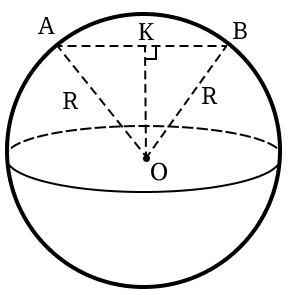
\includegraphics[width=0.2\textwidth]{images/img1}\\
    \end{center}

    1) Проведем $OA$ и $OB$, $\triangle OAB$ - равнобедренный, так как $OA = OB = R$.\\

    2) Проведем $OK \bot AB$, тогда $AK = KB = \frac{m}{2}$, так как $OK$ является высотой и медианой.\\

    3) По теореме Пифагора в $\triangle AKO:$
    \[
        OK = \sqrt {R ^ 2 - \left(\frac{m}{2}\right)^2}
    \]

    Ответ: $\sqrt {R ^ 2 - \left(\frac{m}{2}\right)^2}$

    \begin{center}
        \textbf{№3}
    \end{center}

    Вершины треугольника $ABC$ лежат на сфере радиуса 13 см.
    Найдите расстояние от центра сферы до плоскости треугольника, если $AB = 6$ см, $BC = 8$ см, $AC = 10$ см.

    \textbf{Решение}\\

    \begin{center}
        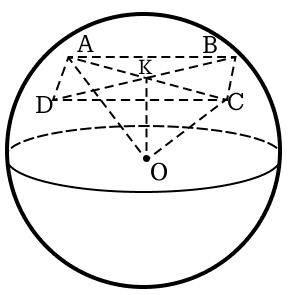
\includegraphics[width=0.2\textwidth]{images/img2}\\
    \end{center}
    1) Заметим, что $\triangle ABC$ - прямоугольный:
    \[ AB ^ 2 + BC ^ 2 = AC ^ 2 \]

    2) Достроим $\triangle ABC$ до прямоугольника $ABCD$, пусть $K$ - точка пересечения диагоналей,
    тогда $DK = BK = AK = CK$

    3) Проведем $OK$, $OA$, $OB$.
    $OA = OB = R$, где $R$ радиус сферы, тогда $\triangle AOC$ - равнобедренный и $OK$ - высота.

    4) Проведем $OD$, $OB$.
    $OD = OB = R$, тогда $\triangle DOB$ - равнобедренный и $OK$ - высота.\\

    5)
    \[\left
        \begin{matrix}
            $DB \cap AC = K$ \\
            $OK \bot DB$     \\
            $OK \bot$ AC     \\
        \end{matrix}\right|\rightarrow OK \bot (ABC) \text{ по признаку перпендикулярности прямой и плоскости}
    \]

    6)
    \[\rho(O; (ABC)) = OK\]
    \[OK = \sqrt{R ^ 2 - AK ^ 2} = \sqrt {13 ^ 2 - 5 ^ 2} =  \sqrt {18 * 8} = 12 \text{ см}\]

    Ответ: 12 см

    \begin{center}
        \textbf{№4}
    \end{center}

    Вершины прямоугольника лежат на сфере радиуса 10 см.
    Найдите расстояние от центра сферы до плоскости прямоугольника, если его диагональ равна 16 см.

    \textbf{Решение}\\

    \begin{center}
        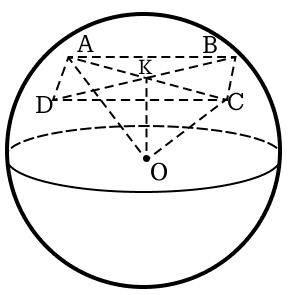
\includegraphics[width=0.2\textwidth]{images/img3}\\
    \end{center}

    1) Пусть $ABCD$ - прямоугольник с диагональю 16 см, а $R=10$ см - радиус сферы, точка пересечения диагоналей $K$,
    $DK = BQ = AK = CK$

    2) Проведем $OK$, $OA= OC = R$, тогда $\triangle AOC$ - равнобедренный, а $OK$ - высота

    3) Проведем  $OB = OD = R$, тогда $\triangle BOD$ - равнобедренный, а $OK$ - высота

    4)
    \[\left
        \begin{matrix}
            $DB \cap AC = K$ \\
            $OK \bot DB$     \\
            $OK \bot$ AC     \\
        \end{matrix}\right|\rightarrow OK \bot (ABC) \text{ по признаку перпендикулярности прямой и плоскости}
    \]

    5)
    \[\rho(O; (ABC)) = OK\]
    \[OK = \sqrt{R ^ 2 - AK ^ 2} = \sqrt {10 ^ 2 - 8 ^ 2} =  \sqrt {2 * 18} = 6 \text{ см}\]

    Ответ 6 см.

    \begin{center}
        \textbf{№5}
    \end{center}

    Расстояние от центра сферы радиуса R до секущей плоскости равно $d$.
    Вычислите:
    \begin{enumerate}
        \item Радиус окружности, полученной в сечении плоскостью, если $R = 5$ см, $d = 3$ см.
        \item Длину окружности, полученной в сечении плоскостью, если $R = 12$ см, $d = 8$ см.
    \end{enumerate}

    \textbf{Решение}\\

    \begin{center}
        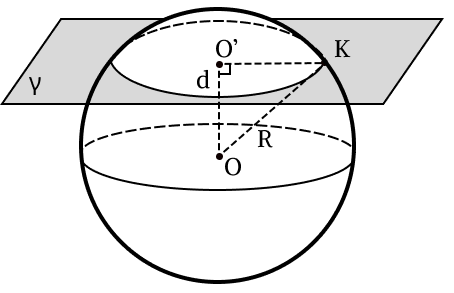
\includegraphics[width=0.2\textwidth]{images/img4}\\
    \end{center}

    \begin{enumerate}
        \item
        \[  O'K =  \sqrt{R ^ 2 - d ^ 2} = \sqrt{5 ^ 2 - 3 ^ 2} = \sqrt {8 * 2} = 4 \text{ см}\]

        \item
        \[  O'K =  \sqrt{R ^ 2 - d ^ 2} = \sqrt{12 ^ 2 - 8 ^ 2} = \sqrt {20 * 12} = 4\sqrt{15} \text{ см}\]
        \[ L = 2\pi r = 8 \pi \sqrt {15} \text{ см}\]
    \end{enumerate}

    Ответ: 1) 4 см; 2) $8 \pi \sqrt {15}$ см

    \begin{center}
        \textbf{№6}
    \end{center}

    Секущая плоскость проходит через конец диаметра сферы радиуса $R$ так,
    что угол между диаметром и плоскостью равен $\alpha$.
    Найдите длину окружности, получившейся в сечении, если:
    \begin{enumerate}
        \item $R = 2$ см, $\alpha = 30 ^{\circ}$;
        \item $R = 5$ см, $\alpha = 45 ^{\circ}$
    \end{enumerate}

     \textbf{Решение}\\

    \begin{center}
        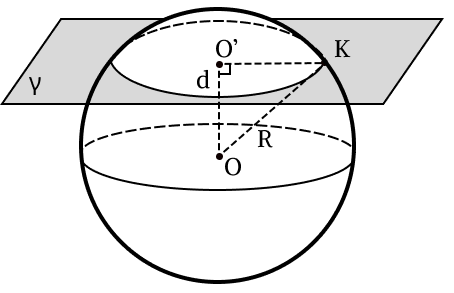
\includegraphics[width=0.2\textwidth]{images/img5}\\
    \end{center}

     \[\angle Q'KO = \alpha , OK = R\]
    \[ r = R * \cos \alpha \]
    \[ L = 2\pi r = 2 \pi R  \cos \alpha \]

    1)
    \[ L = 4\pi \cos 30^{\circ} = \frac{4\sqrt {3}\pi}{2} \] \text{ см}

    2)
    \[
        L = 10 \pi \cos 45^{\circ} = \frac{10\sqrt {2}\pi}{2} \text{ см}
    \]

    Ответ: 1) $\frac{4\sqrt {3}\pi}{2}$ см; 2) $\frac{10\sqrt {2}\pi}{2}$ см

\end{document}
